\chapter{Ultracold Quantum Gases in Optical Lattices}

Ultracold atoms present an extremely powerful tool in quantum reasearch. At the scale of nanokelvins thermal effects no longer destroy the otherwise fragile quantum systems. Thus, quantum phenomena, otherwise only known from theory, can be studied directly. Atomic physics experiments with such ultracold, quantum degenerate gases offer some unique features: (i) a wide range of Hamiltonians can be mapped to the systems making experiments highly customizable. This can in part be attributed to (ii) the very high degree of control achievable through the manipulation of external fields. Through this, the cold atoms can be trapped and manipulated using magnetic and optical traps. Furthermore, the collisional properties of the atoms can be tuned through magnetic Feshbach resonances, and the properties of the gas can be probed through interactions between internal energy levels of the atoms and laser light \cite{JakschZoller, Bloch2012}.\\
In the regime of such cold temperatures many-body phenomena such as Bose-Einstein condensation takes place, where the ground state of a system gains a macroscopic populations. Ever since the first realisation of a Bose-Einstein condensate in 1995 \cite{WiemanCornell1995}, the special properties of this macroscopic quantum state have been used in a wide range of experiments. One method of utilizing Bose-Einstein condensates is to load them into an optical lattice, which is an array of potentials created through the atoms dipole interaction with laser beams. By utilizing the high controllability of these systems, one can perform quantum simulations of various systems, such as spin chains \cite{Simon2011}, Dirac cones \cite{Tarruell2012}, and artificial gauge fields \cite{Dalibard2011}. Furtermore, the properties of cold atoms in optical lattices is very favourable for experiments in quantum information, where quantum gates can be realised through controlled collisions \cite{Zoller1999} or Rydberg atoms \cite{Molmer2010}.\\

\section{Optical Lattice Potentials}
Cold atoms can be trapped in potentials generated by their own dipole interaction with light. Thus, superimposing laser beams allows one to create optical lattices in various shapes and forms. Such dipole traps realised using far-detuned light have important properties, as (i) they are capable of trapping neutral atoms, and (ii) the optical excitation from the trap is very low \cite{grimm}.\\
Optical lattices are a central component of many experiments, as they not only trap the atoms, but also determines many properties of the system.

\subsection{Trapping of Neutral Atoms}
Consider a two level atom in the presence of a time-varying electric field $\boldsymbol{E} = \boldsymbol{\varepsilon} E_0 \exp{ \left( i(\boldsymbol{k} \boldsymbol{r} - \omega_L t) \right)}$, where $E_0$ is its amplitude, $\boldsymbol{\varepsilon}$ is its polarization vector, $\boldsymbol{k}$ is its wave vector and $\omega_L$ is its frequency. The interaction between the atom and the electric field causes a perturbation of the atoms energy levels, otherwise known as the AC Stark-shift. The Hamiltonian describing this interaction is
\begin{equation}
	\hat{H}_{int} = \hat{d} \boldsymbol{E} \; , \label{eq:Hdipint}
\end{equation}
where $\hat{d} = -e \hat{r}$ is the electric dipole operator.\\
Consider equation \eqref{eq:Hdipint} as a perturbation to the Hamiltonian of the atom. To first order the non-degenerate, time-independent perturbation of the energy of state $i$ reads $E_{i}^{(i)} = \bra{i} \hat{H}_{int} \ket{i}$. However, only states of opposite parity will contribute to the matrix elements of $\braket{\hat{H}_{int}}$, as \eqref{eq:Hdipint} is linear in space. Thus, all first-order perturbation terms cancel.\\
To second order the perturbation of state $i$ is given by
\begin{equation}
	E_i^{(2)} = \sum_{j \neq i} \frac{ |\bra{j} \hat{H}_{int}\ket{i}|^2}{\varepsilon_i - \varepsilon_j} \; .
\end{equation}
Here, the states $\ket{i}$ and $\ket{j}$ and their corresponding energies, $\varepsilon_i$ and $\varepsilon_j$, are of the dressed state picture, where one considers the combined system of the atom and the light field \cite{cohen1992atom}. The state $\ket{i}$ represents the atom being in its ground state, while the light field contains $n$ photons. Thus, the energy of the combined state is $\varepsilon_i = n \hbar \omega_L$, when setting the energy of the atomic ground state to zero. Meanwhile, state $\ket{j}$ is when the atom has been excited by absorbing one of the photons of the field. Hence, the energy of this state is $\varepsilon_j = \hbar \omega_0 + (n-1) \hbar \omega_L$. Defining the detuning $\Delta = \omega_L - \omega_0$ allows writing the perturbation in the form
\begin{equation}
	E_{g/e}^{(2)}=\pm  \frac{ |\bra{e}\hat{d}\ket{g}|^2}{\Delta} |E_0|^2,
	\label{2ndpert}
\end{equation}
where the upper sign is assigned to the atomic ground state $\ket{g}$. This can be rewritten in order to reflect properties of the atom and the field, by considering the intensity of the light, $I = \frac{1}{2} \epsilon_0 c |\boldsymbol{E}|^2 $, and the decay rate of the atom, $\Gamma$. Thus, equation \eqref{2ndpert} can be written as \cite{grimm} 
\begin{equation}
	E_{e/g}^{(2)}=\pm \frac{3 \pi c^2}{2 \omega_0} \frac{\Gamma}{\Delta}I
	\label{eq:dipolepot}
\end{equation}
This is the AC-Stark shift, which constitutes the dipole potential. For red detuning ($\Delta < 0$) the ground state will experience a negative shift leading to an attractive potential with depth depending on the intensity of the laser. Similarly, a blue-detuned laser ($\Delta > 0$) will repel the atom. An illustration of this can be seen in figure \ref{fig:ac_stark}.
\begin{figure}[!h]
	\centering
	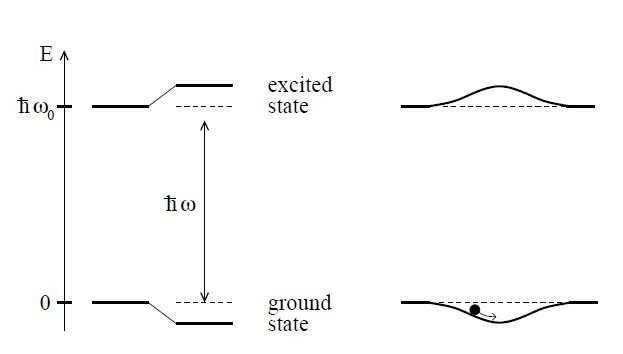
\includegraphics[width=0.5\columnwidth]{Figures/acstark.JPG} 
	\caption{\textit{Light shifts of a two-level atom. Left-hand side,
		red-detuned light ($\Delta < 0$) shifts the ground state down and the
		excited state up by same amounts. Right-hand side, a spatially
		inhomogeneous field like a Gaussian laser beam produces a
		ground-state potential well, in which an atom can be trapped. Figure and 		caption are adopted from \cite{grimm}.}}
	\label{fig:ac_stark} 
\end{figure}
Since the sign is reversed for the excited state, it is important that the atom remains in the ground state. Thus, one has to minimize the scattering with the optical potential. The scattering rate is given as \cite{grimm}
\begin{equation}
	\Gamma_{sc} = \frac{3 \pi c^2}{2 \hbar \omega_{0}^3} \left( \frac{\Gamma}{\Delta} \right) ^2 I \; .
\end{equation}
As the detuning becomes small, the laser becomes resonant with the atom causing a large increase in scattered photons. Therefore, one has to choose a large detuning in order for the potential to remain conservative. However, this comes at the cost of a weaker potential. To compensate this, a high laser intensity must be used, in order for the potential to reach sufficient depth. In practise there will be a limit to the laser power available, however, for most alkali-metal atoms the detuning is typically chosen to be large compared to the excited-state hyperfine structure splitting, which provides enough depth while being sufficient to suppress scattering events \cite{manybodyBloch}. 


\subsection{Optical Lattices}

The dipole potential in equation \eqref{eq:dipolepot} scales with the intensity of the laser. Thus, superimposing laser beams allows for creating a multitude of different potentials through the interference patterns of the lasers. A simple standing wave from two counter-propagating light fields will lead to an array of potential wells
\begin{equation}
	V(z) = - V_0 \cos^2{k z } \; ,
	\label{eq:standwave}
\end{equation}
 where $V_0 = | \frac{3 \pi c^2}{2 \omega_{0}^3} \frac{\Gamma}{\Delta} 4 I_0 |$ from equation \eqref{eq:dipolepot}. In practise, a one dimensional lattice like that of equation \eqref{eq:standwave} is created by shining a single laser beam at a mirror, whereby it interferes with itself.
\begin{figure}[!h]
	\centering
	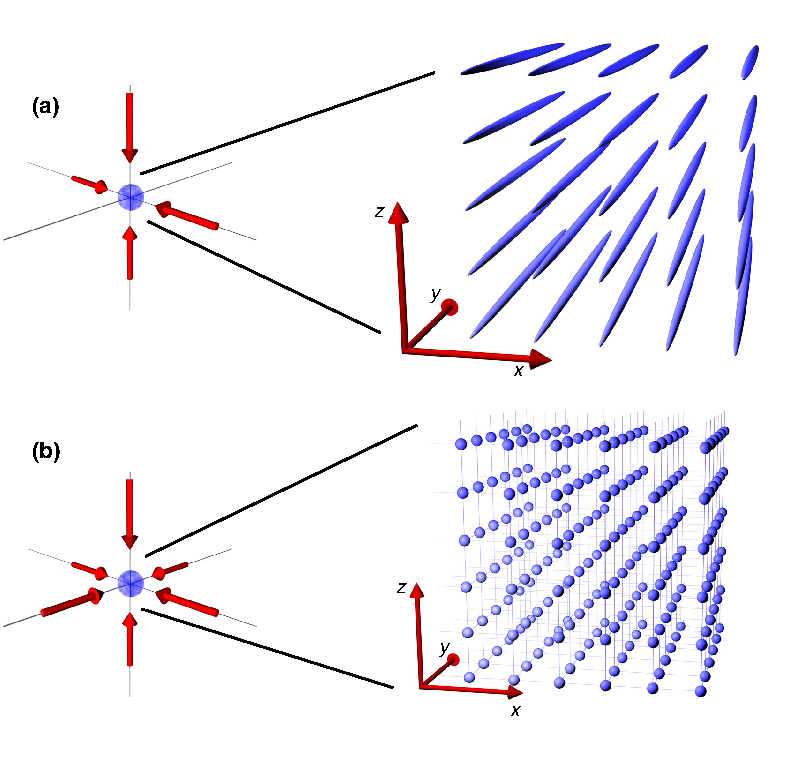
\includegraphics[width=0.8\columnwidth]{Figures/OpticalLattice.pdf} 
	\caption{\textit{\textbf{(a)} Two dimensional optical lattice formed by two mutually orthogonal laser beams. These tubes have a characteristic cigar shape, due to the Gaussian profile of the lasers. \textbf{(b)} Upon using three orthogonal laser beams, the result is a three dimensional lattice reminiscent of a cubic crystal. Figure is adopted from \cite{WideraThesis}.}}
	\label{fig:OpticalLattice} 
\end{figure}
Adding another laser beam in a different direction creates a periodic two dimensional potential. For orthogonal polarization of the two lasers, the resulting potential is purely the sum of the sinusoidal standing wave potential, as no interference term is present \cite{lewenstein}. Note, that the lattice is only well defined for distances much smaller than the waist of the laser beams, as the lattice is only present within the overlap of the two beams. Various shapes of the lattice can be achieved by adjusting the angle between the beams, however, the most common setup is using two orthogonal beam creating a square lattice of one dimensional tubes, as seen in figure \ref{fig:OpticalLattice}.
In order to create a three dimensional lattice, as seen in figure \ref{fig:OpticalLattice}, an additional third perpendicular laser beam is needed. In the center of the trap, the lattice potential is then given by
\begin{equation}
	V(x,y,z) = - V_0 \left( \cos^2{k x } + \cos^2{k y } + \cos^2{k z } \right) \; , \label{eq:3Dlattice}
\end{equation}
for distances much smaller than the beam waist. In addition to the lattice, an external harmonic confinement will be present due to the Gaussian profile of the laser beams \cite{manybodyBloch}.

\subsection{Band Structure}
Consider a periodic potential as described by equation \eqref{eq:standwave}. \textit{Bloch's Theorem} states that energy eigenstates of a periodic potential with lattice vector $\boldsymbol{R}$ and quasi-momentum $q$ can be written as Bloch waves, which takes the form
\begin{equation}
	\phi_{\boldsymbol{q}}^{(n)}(\boldsymbol{r}) = e^{i \boldsymbol{q} \boldsymbol{r}} u^{(n)}(\boldsymbol{r}) \; ,
\end{equation}
which is a plane wave modulated by a function with the same periodicity as the potential $u^{(n)}(\boldsymbol{r}) = u^{(n)}(\boldsymbol{r} + \boldsymbol{R})$. Furthermore, the Bloch waves are periodic in reciprocal space, such that $\psi_{\boldsymbol{q}}^{(n)}(\boldsymbol{r}) = \phi_{\boldsymbol{q} + \boldsymbol{G}}^{(n)}(\boldsymbol{r})$, where $\boldsymbol{G}$ is a reciprocal lattice vector. \cite{kittel} \\
This leads to an energy spectrum in the shape of bands with the periodicity of the first \textit{Brillouin Zone}. Bands are denoted by the band index $n$, and their shape is determined by both the shape and the depth of the potential. The potential depth is often denoted in units of the recoil energy $E_r = \frac{\hbar ^2 k^2}{2 m}$, where $m$ is the mass of the atom, and $k$ is the photon wave number of the light forming the optical lattice. For $V_0 = 0$, the particles are free, hence the bands will be parabolic. Meanwhile, for $V_0 \rightarrow \infty$, no interaction between different wells of the lattice can take place, as the wavefunctions of the trapped atoms will be confined to their respective well. Thus, the lattice is reduced to an array of independent harmonic oscillators, whereby the bands will appear flat with equal spacing \cite{greiner}. 

\subsection{Localized States}
For lattice potential depths within $5 E_r \leq V_0 \leq 8 E_r$, the lattice is in the \textit{tight binding limit}. Within this range, the wavefunctions of the trapped atoms will only overlap with other wells in their closest proximity. Thus, interactions between wells are almost purely of nearest neighbour nature. Due to how well localized the wavefunctions are, a basis of Wannier functions is ideal for describing the system. Wannier functions are related to Bloch functions through the Fourier transform \cite{kittel1963}
\begin{equation}
	w^{(n)}(\boldsymbol{r}) = \frac{1}{\sqrt{N_L}} \sum_{q} e^{ -i \boldsymbol{q} \boldsymbol{R} } \phi_{\boldsymbol{q}}^{(n)}(\boldsymbol{r}) \; ,
\end{equation} 
where $N_L$ is the number of primitive cells of the lattice. The Wannier functions are well localized and centred around the lattice at site $\boldsymbol{R}$. In the case of a separable periodic potential, like that of equation \eqref{eq:3Dlattice}, the single-particle problem becomes dimensional \cite{kohn1959analyticWannier}. Lastly, Wannier functions obey the orthonormality relation
\begin{equation}
	\int \mathrm{d^3}r \; \; w^{(n) *}(\boldsymbol{r} - \boldsymbol{R}) w^{(n')}(\boldsymbol{r} - \boldsymbol{R'}) = \delta_{n,n'} \delta_{\boldsymbol{R},\boldsymbol{R}'} \; ,
\end{equation}
thus forming a complete basis \cite{manybodyBloch}. 
\begin{figure}[!h]
	\centering
	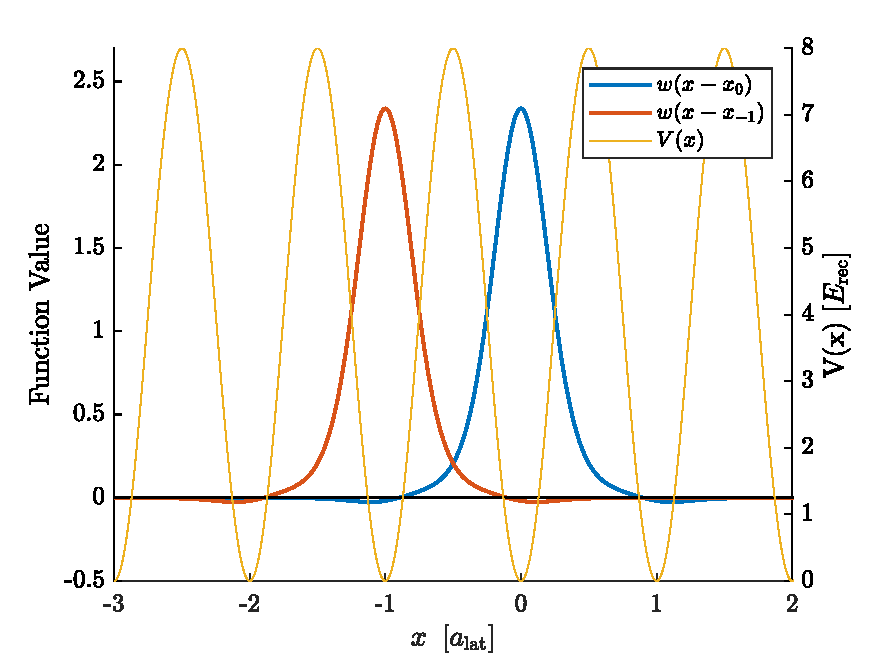
\includegraphics[width=0.8\columnwidth]{Figures/WannierPlot3.pdf} 
	\caption{\textit{Two one-dimensional Wannier functions plotted for a lattice potential depth of $V_0 = 8 E_r$.}}
	\label{fig:WannierPlot} 
\end{figure}
Figure \ref{fig:WannierPlot} shows Wannier functions plotted for lattice potential depths within the tight binding limit. As evident from the plot, the functions overlap with only their nearest neighbours. In the case of a more shallow lattice, the functions would extends to further wells, while they will tend towards a Gaussian shape as the lattice depth increases \cite{greiner}.



\section{Bose-Einstein Condensates}

Bosons are particles of integer spin, whose statistics obey those of a Bose-Einstein distribution
\begin{equation}
	n_i = \frac{g_i}{\exp \left( \left( \varepsilon_i -\mu \right) / k_B T \right) - 1} \; , \label{eq:BHdistribution}
\end{equation} 
where $i$ denotes the state, $n_i$ is the population of the state, $g_i$ is its degeneracy, $\varepsilon_i$ is its energy, $\mu$ is the chemical potential, $k_B$ is the Boltzmann constant, and $T$ is the temperature. One important feature of bosons is that, unlike fermions, multiple particles can occupy the same quantum state. At higher temperatures the energy spectrum is practically continues, whereby this property has little effect, as two particles occupying the same single-particle state is highly unlikely. However, at low temperatures the energy spectrum systems often become increasingly discrete, hence the statistics of the particles becomes very important. As evident from equation \eqref{eq:BHdistribution}, the population of the ground state diverges as $T \to 0$. However, even below the finite temperature, $T_c$, one will observe a macroscopic population of the ground state. $T_c$ is called the critical temperature, and marks the point where multiple particles will start forming a Bose-Einstein Condensate (BEC). \cite{pethick2002bose}

\subsection{Non-Interacting Particles}
In the case of non-interacting particles and zero temperature, all particles of a Bose gas can be described by identical single-particles wavefunctions $\phi (\boldsymbol{r}_i)$. Hence, the many-body wavefunction is simply given by the product 
\begin{equation}
	\Psi (\boldsymbol{r}_1 , \ldots , \boldsymbol{r}_N) = \prod_{i}^{N} \phi (\boldsymbol{r}_i) \; .
\end{equation}
Such a product state can be described by a single macroscopic wavefunction
\begin{equation}
	\psi (\boldsymbol{r}) = \sqrt{N} \varphi (\boldsymbol{r}) \; , \label{eq:psi_NIBEC}
\end{equation}
where $\phi (\boldsymbol{r})$ is the wave function of the single-particle state, in which the bosons condensate into \cite{PenroseOnsager}.

\subsubsection{Second-Quantization}
When describing Bose-Einstein condensates it is very convenient to work in second quantization, which describes the number of particle in each state rather than the state of each particle.\\
First, consider a basis of single particle states $\{ \ket{n} \}$, namely a Fock basis. In this space particles are created or annihilated through their respective operators
\begin{equation}
	\hat{a}_{\mu}^{\dag} \ket{0_\mu} = \ket{1_\mu} \; .
\end{equation}
For bosons the creation and annihilation operators fulfill the commutation relations
\begin{equation}
[\hat{a}_\nu,\hat{a}_\mu]=[\hat{a}_\nu^\dagger,\hat{a}_\mu^\dagger]=0 \quad , \quad [\hat{a}_\nu,\hat{a}_\mu^\dagger]=\delta_{\nu,\mu} \; , 
\end{equation}
with the number operator given as
\begin{equation}
	\hat{n}_{\mu} = \hat{a}_{\mu}^{\dag} \hat{a}_{\mu} \; .
\end{equation}
In second quantization many-body states are described by the occupation of the individual Fock states. Thus, a creation operator will raise the number of particles in its corresponding state by one, while the annihilation operator will lower it:
\begin{align}
\hat{a}^\dagger \ket{N_0,N_1, \ldots , N_{\nu},\ldots}&= \sqrt{N_\nu+1}\ket{N_0,N_1, \ldots , N_{\nu}+1,\ldots} \\
\hat{a} \ket{N_0,N_1, \ldots , N_{\nu},\ldots}&= \sqrt{N_\nu}\ket{N_0,N_1, \ldots , N_{\nu}-1,\ldots} .
\end{align}
Likewise, the number operator $\hat{n}_{\mu}$ will count the number of particles in its corresponding state.\\
These operators can be combined with an orthonormal basis of spatial wavefunctions $\{ \phi_k \}$ in order to create field operators
\begin{equation}
	\hat{\psi}(\boldsymbol{r}) = \; \sum_{k} \phi_k \hat{a}_{k} \quad , \quad \hat{\psi}^{\dag}(\boldsymbol{r}) = \; \sum_{k} \phi_{k}^{*} \hat{a}_{k}^{\dag} \; ,
\end{equation}
where $\hat{\psi}(\boldsymbol{r})$ will create a particle at location $\boldsymbol{r}$. For bosons the field operators fulfil the commutation relations \cite{bruus}
\begin{equation}
	\left[ \hat{\psi}(\boldsymbol{r}) \; , \; \hat{\psi}^{\dag}(\boldsymbol{r'}) \right] = \; \delta(\boldsymbol{r} - \boldsymbol{r}') \quad , \quad
	\left[ \hat{\psi}(\boldsymbol{r}) \; , \; \hat{\psi}(\boldsymbol{r'}) \right] = \; 0 \; .
\end{equation}
Now, consider a gas of non-interacting bosons described by equation \eqref{eq:psi_NIBEC}, where $\epsilon_k$ is the energy of the $k$'th single-particle state. Due to the completeness of the basis of single-particle wavefunctions, $\{ \phi_k \}$, the creation operator can be expressed as
\begin{equation}
	\hat{a}_k = \int \mathrm{d^3} r \;  \phi_{k}^*(\boldsymbol{r}) \hat{\psi}(\boldsymbol{r}) \; .
\end{equation}
Using this, the Hamiltonian can be written as
\begin{align}
	\hat{H}^{(0)} =& \; \sum_{k} \epsilon_k \hat{a}_{k}^{\dag} \hat{a}_{k} \nonumber \\
		=& \;  \sum_{k} \int \mathrm{d^3}r_1 \mathrm{d^3}r_2 \; \epsilon_k \phi_k (\boldsymbol{r_1}) \phi_{k}^* (\boldsymbol{r_2})\; \; \hat{\psi}^{\dag} (\boldsymbol{r_1}) \hat{\psi} (\boldsymbol{r_2}) \nonumber \\
		=& \; \int \mathrm{d^3}r  \; \hat{\psi}^{\dag}(\boldsymbol{r}) \left( - \frac{\hbar^2}{2 m} \nabla^2 + U(\boldsymbol{r})\right) \hat{\psi}(\boldsymbol{r})
		\label{hamil2nd}
\end{align}

\subsection{Weakly Interacting Particles}
A characteristic of a BEC is its low temperature and density. Thus, is it a valid approximation to only consider two-particle interactions
\begin{equation}
	\hat{H}^{(2)} = \frac{1}{2} \sum_{i \neq j} V(\boldsymbol{r_i} - \boldsymbol{r_j}) \; .
\end{equation}
At low energies all interactions can be considered of s-wave nature, because
all waves of higher angular momentum are reflected by the centrifugal barrier. Furthermore, for cold gases the thermal de Broglie wavelength is much larger than the effective extension of the interaction potential. Therefore, the actual shape of the scattering potential is irrelevant, hence one can replace it with a pseudo-potential
\begin{equation}
	V(\boldsymbol{r} - \boldsymbol{r'}) = g \; \delta(\boldsymbol{r} - \boldsymbol{r'}) = \frac{4 \pi \hbar^2 a}{m} \delta(\boldsymbol{r} - \boldsymbol{r'}) \; ,
\end{equation}
which results in the same scattering phase as the real, more complicated scattering potential. Thus, the interaction of cold atoms is fully determined by the scattering length, $a$ \cite{greiner}.\\
Introducing the density operator
\begin{equation}
	\hat{\rho}(\boldsymbol{r}) = \hat{\psi}^{\dag}(\boldsymbol{r}) \hat{\psi}(\boldsymbol{r}) \; ,
\end{equation}
allows writing $\hat{H}^{(2)}$ in second quantization
\begin{align}
	\hat{H}^{(2)} &= \frac{1}{2} \int \mathrm{d^3}r_1 \mathrm{d^3}r_2 V(\boldsymbol{r_1} - \boldsymbol{r_2}) \hat{\psi}^{\dag}(\boldsymbol{r_1}) \hat{\psi}(\boldsymbol{r_1}) \left( \hat{\psi}^{\dag}(\boldsymbol{r_2}) \hat{\psi}(\boldsymbol{r_2}) - \delta(\boldsymbol{r_1} - \boldsymbol{r_2}) \right) \\
	&= \frac{1}{2} \int \mathrm{d^3}r_1 \mathrm{d^3}r_2  \hat{\psi}^{\dag}(\boldsymbol{r_1}) \hat{\psi}^{\dag}(\boldsymbol{r_2}) V(\boldsymbol{r_1} - \boldsymbol{r_2}) \hat{\psi}(\boldsymbol{r_1}) \hat{\psi}(\boldsymbol{r_2}) \; .
\end{align}
Combining this with the basic Hamiltonian of equation \eqref{hamil2nd}, gives the full Hamiltonian in second quantization
\begin{align}
	\hat{H} &= \hat{H}^{(0)} + \hat{H}^{(2)} \\
	& = \int \mathrm{d^3}r \ \hat{\psi}^{\dag}(\boldsymbol{r}) \left( - \frac{\hbar^2}{2 m} \nabla^2 + U(\boldsymbol{r})\right) \hat{\psi}(\boldsymbol{r}) + \frac{1}{2} \int \mathrm{d^3}r_1 \mathrm{d^3}r_2  \ \hat{\psi}^{\dag}(\boldsymbol{r_1}) \hat{\psi}^{\dag}(\boldsymbol{r_2}) V(\boldsymbol{r_1} - \boldsymbol{r_2}) \hat{\psi}(\boldsymbol{r_1}) \hat{\psi}(\boldsymbol{r_2})
	\label{hamilint}
\end{align}
Using this Hamiltonian to try and solve the Heisenberg equations of motion for the field operators leads to
\begin{equation}
	i \hbar \frac{\partial }{\partial t} \hat{\psi}(\boldsymbol{r}) = \left[ \hat{\psi}(\boldsymbol{r}) \; , \; \hat{H}  \right] = \left( - \frac{\hbar^2}{2 m} \nabla^2 + U(\boldsymbol{r}) + g \hat{\psi}^{\dag}(\boldsymbol{r}) \hat{\psi}(\boldsymbol{r}) \right) \hat{\psi}(\boldsymbol{r}) \; ,
\end{equation}
which is not solvable in general. However, in the scenario of a BEC the scattering length $a$ is much less than the mean inter-particle distance, such that $n a^3 \ll 1$, where $n$ is the density of the gas. In this regime the mean-field approximation is viable
\begin{equation}
	\hat{\psi}(\boldsymbol{r}) = \psi(\boldsymbol{r}) + \delta \hat{\psi}(\boldsymbol{r}) \; ,
\end{equation}
where $\psi(\boldsymbol{r})$ is the mean-field given by equation \eqref{eq:psi_NIBEC}, and $\delta \hat{\psi}(\boldsymbol{r})$ is fluctuations from the mean. If $\braket{\delta \hat{\psi}(\boldsymbol{r})} = 0$, the fluctuations can be neglected, leading to the Gross-Pitaevskii equation \cite{Gross1961,Pitaevskii}
\begin{equation}
	i \hbar \frac{\partial }{\partial t} \hat{\psi}(\boldsymbol{r}) = \left( - \frac{\hbar^2}{2 m} \nabla^2 + U(\boldsymbol{r}) + g |\psi(\boldsymbol{r})|^2 \right) \psi(\boldsymbol{r}) \; .
\end{equation}
The Gross-Pitaevskii equation is very similar to the Schrödinger equation with exception of the non-linear term $g |\psi(\boldsymbol{r})|^2$, which can make the equation hard to solve in regions of low density.



\section{Bose-Hubbard Model of Interacting Bosons in a Lattice}
The Bose-Hubbard model describes weakly interacting bosons in a periodic lattice within the tight binding limit. The model is perfectly capable of predicting results with good accuracy, however, two conditions must hold in order for the it to be valid: (i) both the thermal energy and the mean interaction energy at a single site must be much smaller than the separation to first excited band, $\hbar \omega_0$, and (ii) the Wannier functions decay essentially within the length of the lattice constant \cite{manybodyBloch}.\\
Under these conditions one is assured that only the lowest band is taken into account, and that only nearest-neighbour interactions take place.\\
The Bose-Hubbard model is interesting, as it supports two distinct phases: the Superfluid phase and the Mott-Insulator phase. Furthermore, the model contains effects such as a quantum phase transition between the two phases mentioned above, which can be crossed without any change in external parameters. 


\subsection{The Bose-Hubbard Hamiltonian}
Consider the Hamiltonian for bosonic particles in a trapping potential (described by equation \eqref{hamilint}) in one dimension. For a periodic lattice potential in the tight binding limit it is favourable to work in a basis of localized Wannier functions. Expanding the field operators of the Hamiltonian in equation \eqref{hamilint} in  the Wannier basis yields \cite{Jaksch}
\begin{align}
	\hat{H} &= \int \mathrm{d}x \sum_{i j} w^*(x-x_i) \hat{a}_{i}^{\dag} \left( - \frac{\hbar^2}{2 m} \nabla ^2 + V(x) \right) w(x-x_j) \hat{a}_j \nonumber \\
	& \quad + g \int \mathrm{d}x \sum_{i j k l} w^*(x-x_i) w^*(x-x_j) w(x-x_k) w(x-x_l) \hat{a}_{i}^{\dag} \hat{a}_{j}^{\dag} \hat{a}_{k} \hat{a}_{l} \\
	&= - \sum_{i j } J_{i j} \hat{a}_{i}^{\dag} \hat{a}_{j} + \sum_{i j k l} U_{i j k l} \hat{a}_{i}^{\dag} \hat{a}_{j}^{\dag} \hat{a}_{k} \hat{a}_{l} \; ,
\end{align}
where
\begin{align}
	J_{i j} &= - \int \mathrm{d}x \ w^*(x-x_i) \left( - \frac{\hbar^2}{2 m} \nabla ^2 + V(x) \right) w(x-x_j) \\
	U_{i j k l} &= g \int \mathrm{d}x \ w^*(x-x_i) w^*(x-x_j) w(x-x_k) w(x-x_l) 
	\label{eq:BHparamJ}
\end{align}
Since the system is periodic, one can consider a single site, $i = 0$, as representative for the entire lattice. In this way, the different terms of the Hamiltonian can be interpreted as follows:
\begin{align}
	J_{0 0} &= \text{constant energy offset} \nonumber \\
	J_{0 1} &= \text{"overlap matrix element" to neighbouring site} \nonumber \\
	J_{0 2 - 0 \infty} &= \text{"overlap matrix element" to further sites} \nonumber \\
	U_{0 0 0 0} &= \text{on-site interaction for two particles} \nonumber \\
	U_{0 i i 0} &= \text{interaction off-site} \nonumber \\
	U_{0 0 0 1} &= \text{interaction  + tunnelling , off-site} \nonumber 
\end{align}
Due to the rapid decay of the Wannier functions, the overlap of wavefunctions is limited to their nearest neighbour. Dropping all exponentially suppressed terms and constant offsets yields the Bose-Hubbard Hamiltonian
\begin{equation}
	\hat{H} = - J \sum_{\langle i,j \rangle} \hat{a}_{i}^{\dag} \hat{a}_{j} + \frac{U}{2} \sum_{i} \hat{n}_i \left( \hat{n}_i -1 \right) + \sum_{i} \varepsilon_i \hat{n}_i \; ,
	\label{BHhamil}
\end{equation}
where $J = J_{0 1}$, $\langle i,j \rangle$ only counts neighbouring pairs, and
\begin{equation}
	U = U_{0 0 0 0} = g \int \mathrm{d}x \ |w(x)|^4 \; .
	\label{eq:BHparamU}
\end{equation}
The first term of the Bose-Hubbard Hamiltonian describes the kinematics within the model, which takes the form of tunneling between neighbouring sites. This is interpreted by annihilating a particle at site $j$ while creating a particle at site $i$. The second term describes the interaction between particles within a single site, and the last term $\sum_{i} \varepsilon_i \hat{n}_i$ takes into account a possible potential offset at different sites.


\subsection{Phases of the Bose-Hubbard Model}

The Bose-Hubbard model supports two quantum phases: The \textit{Superfluid} phase and the \textit{Mott Insulator} phase. These phases depend on the ratio $J/U$, and can be described separately by examining the ground state of the Bose-Hubbard Hamiltonian in the two extreme limits of the $J/U$ ratio.

\subsubsection{Superfluid Phase}
For a system where the tunneling matrix element $J$ is dominant, the lowest energy is obtained by delocalizing the atoms over the entire lattice. Thereby the wavefunction will be a product over single-particle states, and the system will be a superfluid \cite{greiner}.\\
Consider the case of negligible interactions and a lattice of equal depth. In this scenario the Bose-Hubbard Hamiltonian reduces to
\begin{equation}
	\hat{H} = \hat{H}_J = - J \sum_{\langle i,j \rangle} \hat{a}_{i}^{\dag} \hat{a}_{j} \; , 
	\label{hamilSF}
\end{equation}
which is completely periodic within the lattice due to the lack of site specific terms. This leads to solutions in the shape of Bloch waves. The Fourier transform of the annihilation and creation operators
\begin{equation}
	\hat{a}_j = \frac{1}{N_L} \sum_{q}  e^{i q x_j} \hat{a}_q \quad , \quad
	\hat{a}_{j}^{\dag} = \frac{1}{N_L} \sum_{q}  e^{-i q x_j} \hat{a}_{q}^{\dag}
\end{equation}
allows for writing the Hamiltonian \eqref{hamilSF} in momentum space
\begin{equation}
	\hat{H}_J = - J \sum_{q = - \infty}^{\infty} \left( e^{- i q d } + e^{i k d} \right) \hat{n}_q \; ,
\end{equation}
where $d$ is the lattice distance. In momentum space the Hamiltonian is diagonal and results in a continuous energy spectrum
\begin{equation}
	E_q = -2 J \cos(q d) \; .
	\label{SFenergy}
\end{equation}
Thus, the excitation spectrum of the Superfluid is said to be gapless.

The lowest energy is of the system is obtained for $q = 0$, whereby the ground state is
\begin{equation}
	\ket{\Psi_{SF}} =  \frac{1}{\sqrt{N!}} \left( \hat{a}_{q = 0}^{\dag} \right) ^N \ket{0} = \frac{1}{\sqrt{N!}} \left( \frac{1}{N_L} \sum_{j = 1}^{N_L} \hat{a}_{j}^{\dag} \right) ^N \ket{0} \; ,
\end{equation} 
where $N$ is the number of particles. This state supports a well defined macroscopic phase on each lattice site, since the many-body state is a product over identical single-particle states \cite{greiner}. With all particle condensed into the $q = 0$ momentum space state, the particles are completely de-localized in real space, which can be seen by taking the Fourier transform. For large $N,N_L \rightarrow \infty$ at fixed density $N/N_L$ the state becomes indistinguishable from having coherent states, $\ket{\alpha} $, on all lattice sites \cite{manybodyBloch}
\begin{equation}
	\ket{\Psi_{SF}} \approx \prod_j \left( e^{\sqrt{N/N_L} \hat{a}_{j}^{\dag}} \right) \ket{0} = \ket{\alpha_1} \otimes \ket{\alpha_2} \otimes \ldots
	\label{stateSF}
\end{equation}
\begin{figure}[!h]
	\centering
	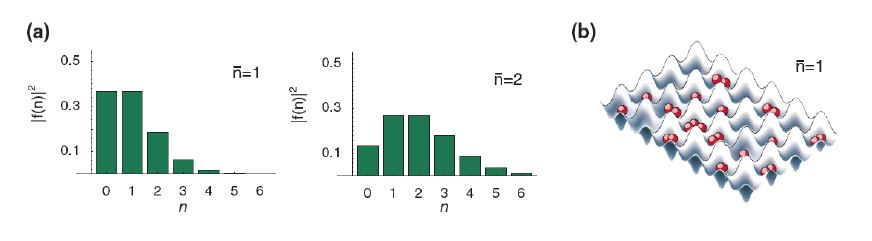
\includegraphics[width=0.8\columnwidth]{Figures/f(n)_SF.JPG} 
	\caption{\textbf{(a)}The statistics for the number of particles per lattice site $n$ for a filling fraction of $\bar{n}=1$ and $\bar{n}=2$ in the superfluid phase. \textbf{(b)} Illustration of the particles in the lattice. There will be large fluctuations of the number of particles found at each lattice site at a given time. Figure and caption adopted from \cite{greiner}.}
	\label{fig:f(n)_SF} 
\end{figure}
Since bosonic operators at different sites commute, the superfluid state can be factorized into a product of local coherent states.
Coherent states are eigenstates of the annihilation operator $\hat{a} \ket{\alpha} = \alpha \ket{\alpha}$, where $|\alpha |^2$ can be considered the particle density of the system, and $\alpha = |\alpha| e^{i \phi}$, with $\phi$ being a global phase. Utilizing the coherent state form of the wavefunction (eq. \eqref{stateSF}) the average filling fraction $\bar{n}$ can be calculated
\begin{equation}
	\bar{n} = \braket{\hat{n}_i} = \bra{\Psi_{SF}} \hat{a}_{j}^{\dag} \hat{a}_{j} \ket{\Psi_{SF}} = \frac{N}{N_L} \; ,
\end{equation}
as well as the fluctuations of particle number per site
\begin{equation}
	\frac{\sqrt{\Delta \bar{n}^2}}{\bar{n}} \sim \frac{1}{\sqrt{\bar{n}}} \; .
\end{equation}
Therefore, the probability distribution for the number of atoms at a given site is Poissonian, which can be seen in figure \ref{fig:f(n)_SF}. Due to the relatively large fluctuation of particle number per site, one would find a somewhat random number of atoms at a given site in a measurement. In the presence of a finite interaction, $U$, the resulting distribution would be sub Poissonian due to number squeezing \cite{greiner}.


\subsubsection{Mott-Insulator Phase}
In the case of negligible tunneling, only the on-site interaction between the atoms has to be taken into account, and the Bose-Hubbard Hamiltonian reduces to
\begin{equation}
	\hat{H} = \hat{H}_U = \frac{U}{2} \sum_{i} \hat{n}_i \left( \hat{n}_i -1 \right) \; ,
	\label{hamilMott}
\end{equation}
which is quadratic in $\hat{n}_i$. This heavily penalizes having multiple particles at the same site. Thus, the ground state of the system will be an equal distribution of all the particles throughout the lattice. Any fluctuations from this average will increase the energy, whereby the phase is said to be incompressible \cite{Gemelke2009}. This incompressibility can be formulated as $\frac{\partial n}{\partial \mu} = 0$, where $\mu$ is the chemical potential, and is the defining property of the Mott-Insulator \cite{manybodyBloch}.\\
\begin{figure}[!h]
\centering
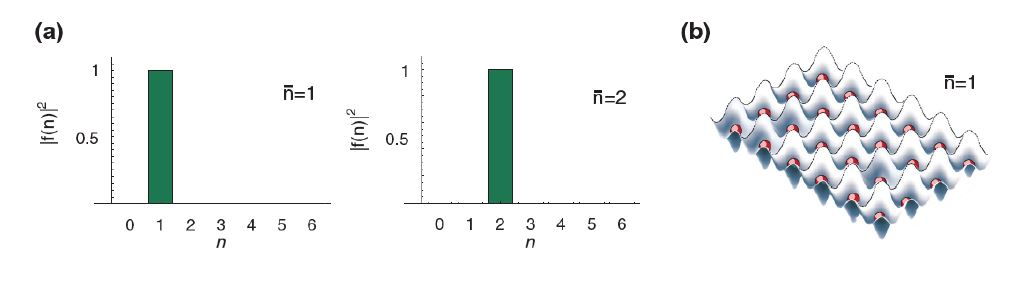
\includegraphics[width=0.8\columnwidth]{Figures/f(n)_M.JPG} 
\caption{\textbf{(a)}The statistics for the number of particles per lattice site $n$ in the Mott-insulator phase, for a filling fraction of $\bar{n}=1$ and $\bar{n}=2$. \textbf{(b)} Illustration of the particles in the lattice. The particles does not hop around in the lattice and are equally distributed. Caption and figure are adapted from \cite{greiner}.}
\label{fig:f(n)_M} 
\end{figure}
Consider the case $\bar{n} = 1$, (average filling of one particle per site). This can be described by a state with a single particle located on each site \cite{manybodyBloch}
\begin{equation}
	\ket{\Psi_{Mott}} = \prod_j \hat{a}_{j}^{\dag} \ket{0} \; .
	\label{eq:MIstate}
\end{equation}
This is a simple product of local Fock states with precisely
one atom per site, which is illustrated in figure \ref{fig:f(n)_M}. This is the configuration of atoms, which minimizes the energy with regards to the Hamiltonian of eq. \eqref{hamilMott}. Any fluctuation from unit occupancy will increase the energy, as merely a single double occupancy will increase the energy by $U$. Thereby, unlike the energy spectrum of the Superfluid, the Mott-Insulator spectrum is gapped. As long as the gain in kinetic energy due to hopping, $J$, is smaller than the on-site interaction, $U$, the atoms remain localized. However, for $J > 0$ the ground state is no longer a the simple product state described in eq. \eqref{eq:MIstate} \cite{manybodyBloch}. As $J$ increases, the gap in the excitation spectrum will gradually decrease until the transition to the superfluid is reached and the spectrum becomes gapless.\\
While the Mott-Insulator phase has complete localization, the phases on the individual sites have obtained maximum uncertainty. Therefore, no phase coherence between different sites is present \cite{greiner}.


\subsection{Phase Transition}
Consider once again the full Bose-Hubbard Hamiltonian \eqref{BHhamil}. The superfluid and the Mott-Insulator account for the two limits of the ratio $J/U$, however, it order to understand the full phase diagram of the Bose-Hubbard model one has to derive the $U_{crit}$ for which the phase transition occurs. There are several ways of doing this - one of them is looking at a mean-field solution of the Bose-Hubbard model. For simplicity the scenario $T=0$ is treated here. Even without a change of temperature the phase transition still happens, hence the label \textit{quantum phase transition} referring to the fact that the phase transition can happen without change of external parameters \cite{Sachdev2007QPT}.\\
Applying the mean field approximation to the annihilation operator yields
\begin{equation}
	\hat{a}_j = \psi + \delta \hat{a}_j \; ,
\end{equation}
where $\psi$ is the locally constant mean field, and $\delta \hat{a}_j$ is the fluctuation term. Inserting this into the Hamiltonian yields
\begin{equation}
	\hat{H}_{MF} = -J \sum_{\langle i,j \rangle} \left( \psi^* + \delta \hat{a}_{i}^{\dag} \right) \left( \psi + \delta \hat{a}_{j} \right) + \text{int.}
\end{equation}
Instead of considering the Hamiltonian as a whole, it can be considered as a sum of local on-site Hamiltonians
\begin{equation}
	\hat{H}_{MF} = \sum_{i} \hat{h}_i \; .
\end{equation}
For a homogeneous system $\hat{h}_i = \hat{h}_j \; \; \forall i,j$. One can write the kinetic part of the Hamiltonian locally if one assumes small fluctuations from the mean field
\begin{align}
  \hat{a}_{i}^{\dag} \hat{a}_{j} &= \left( \psi^* + \delta \hat{a}_{i}^{\dag} \right) \left( \psi + \delta \hat{a}_{j} \right) \nonumber \\
  &= \psi^* \psi + \psi^* \delta \hat{a}_j + \psi \delta \hat{a}_{i}^{\dag} + \delta \hat{a}_{i}^{\dag} \delta \hat{a}_{j} \nonumber \\
  & \approx \psi^* \psi + \psi^* \left( \hat{a}_j - \psi \right) + \psi \left( \hat{a}_{i}^{\dag} - \psi^* \right) \nonumber \\
&= \psi^* \hat{a}_j + \psi \hat{a}_{i}^{\dag} - \psi^* \psi
\end{align}
Since every term only contains a single index, one can let $j \rightarrow i$ leaving a local description
\begin{equation}
	\hat{h}_i = J z \psi^* \psi - J z \left( \psi^* \hat{a}_i + \psi \hat{a}_{i}^{\dag} \right) + \frac{U}{2} \hat{n}_i \left( \hat{n}_i -1 \right) + \mu_i \hat{n}_i \; ,
	\label{localhamil}
\end{equation}
where $z$ is the number of neighbours of site $i$ \cite{vanoosten}. The last term added is a chemical potential, which is needed due to the lack of a fixed particle number locally prompting the use of a Grand Canonical Ensemble description.\\
Landau theory is a general theory regarding phase transitions, which states that in the vicinity of a critical point, one may expand the free energy in a power series of some order parameter $m$. Thus, in order to find $U_{crit}$, equation \eqref{localhamil} must be minimized. In this case this order parameter is the mean field, hence
\begin{equation}
	E_{MF} = \text{const. } + a |\psi|^2 + b |\psi|^4 + \ldots \label{eq:landau}
\end{equation} 
Plotting this yields an effective potential, seen in figure \ref{fig:landau}, which dictates certain properties of the system.
\begin{figure}[!h]
\centering
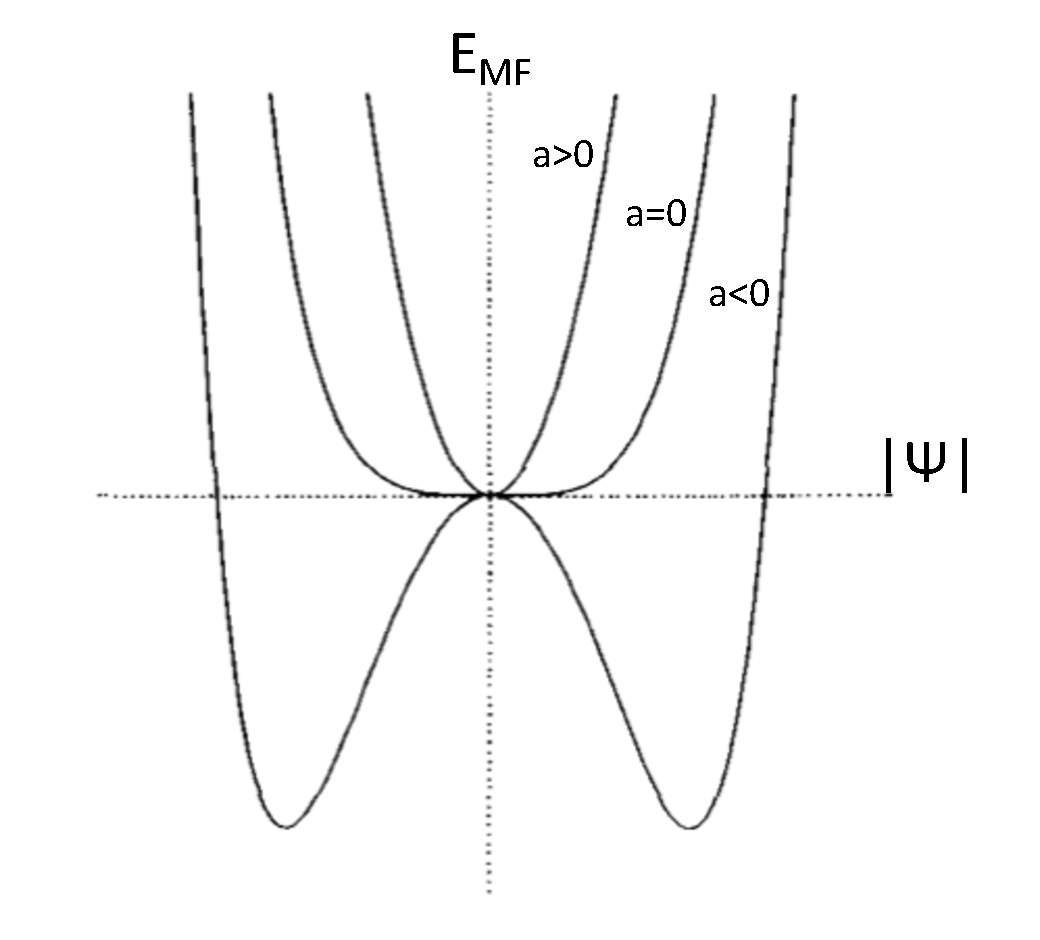
\includegraphics[width=0.7\columnwidth]{Figures/Landau_theory.pdf} 
\caption{	\textit{Effective potential as function of the order parameter $\psi$. For $a<0$ the properties of the potential change from having a single, central minimum to having two separated minima. This is an example of spontaneous symmetry breaking associated with a phase transition. \cite{plischke}}}
\label{fig:landau} 
\end{figure} 

The potential is symmetric in the complex plane allowing the system to have any phase. Furthermore, at some critical value of $a$, (here $a = 0$), the potential will shift from having a single central minimum to having minima at some $|\psi|$. This is a U(1) spontaneous symmetry breaking, which in Landau theory is associated with a phase transition \cite{plischke}. Thus, one need to compute the parameter $a$ of equation \eqref{eq:landau}.\\
One method is using second order perturbation theory, where the $\hat{\psi} = 0$ case is solved exactly, followed by adding a small $\hat{\psi}$ as a perturbation
\begin{equation}
	\hat{h}_{i}^{(0)} = J z \left( \psi^* \psi \right) + \frac{U}{2} \hat{n}_i \left( \hat{n}_i -1 \right) - \mu \hat{n}_i \; .
\end{equation} 
Since the zero-order solution only contain number operators, the ground state of the solution can be expressed in the Fock basis:
\begin{align*}
	\ket{0} \quad &\text{for} \quad \mu < 0 \\
	\ket{1} \quad &\text{for} \quad 0 \leq \mu < U \\
	\ket{2} \quad &\text{for} \quad U \leq \mu < 2 U \\
	& \vdots
\end{align*} 
Adding on the first order perturbation to the energy
\begin{equation}
	E_{i}^{(1)} = \bra{n} \delta \hat{a}_i \ket{n} = 0 \; ,
\end{equation}
yields nothing, thus requiring the use of a second order perturbation
\begin{equation}
	E_{i}^{(2)} = \sum_{n \neq g} \frac{|\bra{n} \delta \hat{h}_i \ket{g}|^2}{E_{g}^{(0)} - E_{n}^{(0)}} \; .
\end{equation}
Here the perturbation Hamiltonian
\begin{equation}
	\hat{h}_i = - z J \left( \hat{a}_i \psi^* + \psi \hat{a}_{i}^{\dag} \right)
\end{equation}
contains only single creation/annihilation operators, whereby
\begin{equation}
	\bra{n} \delta \hat{h}_i \ket{g} = 0 \quad \text{for} \quad |n - g| \neq 1 \; .
\end{equation}
Hence, for each annihilation and creation operator only two matrix elements will give a contribution
\begin{align*}
	\bra{n}  \hat{a}_{i}^{\dag} \ket{n-1} &= \sqrt{n} \braket{n|n} \\
	\bra{n+1}  \hat{a}_{i}^{\dag} \ket{n} &= \sqrt{n+1} \braket{n|n} \\
	& \vdots
\end{align*}
With this the second order perturbation energy reduces to
\begin{align}
	E_{i}^{(2)} &= \left( J z \right)^2 |\psi|^2 \left( \frac{n}{E_{g}^{(0)}- E_{n-1}^{(0)}} +  \frac{n+1}{E_{n}^{(0)}- E_{n+1}^{(0)}} \right) \nonumber \\
	&= \left( J z \right)^2 |\psi|^2 \left( \frac{n}{U(n-1) - \mu} + \frac{n+1}{\mu - U n} \right) \; .
\end{align}
Since $a$ is the pre-factor of all terms proportional $|\psi|^2$, collecting those across from all the perturbations yields the approximation 
\begin{equation}
	a = J z + \left( J z \right)^2 |\psi|^2 \left( \frac{n}{U(n-1) - \mu} + \frac{n+1}{\mu - U n} \right) \; .
\end{equation} 
As stated earlier $U_{crit}$ can be found from $a = 0$:
\begin{equation}
	0 \overset{!}{=} 1 + \frac{n}{\bar{U} (n-1) - \bar{\mu}} + \frac{n+1}{\bar{\mu} - \bar{U} n} \; ,
\end{equation}
with $\bar{mu} = \frac{\mu}{J z}$ and $\bar{U} = \frac{U}{J z}$. Finally, the solution for the chemical potential is \cite{vanoosten}
\begin{equation}
	\bar{mu}_{\pm} = \frac{1}{2} \left( \bar{U}(2n -1) \pm \frac{1}{2} \sqrt{\bar{U}^2 - 2 \bar{U} (2 n +1)} \right) \; .
\end{equation}
Understanding this result can be done be examining figure \ref{fig:SFMOTT}, which displays a phase diagram of the Bose-Hubbard model.  
\begin{figure}[h]
	\centering
	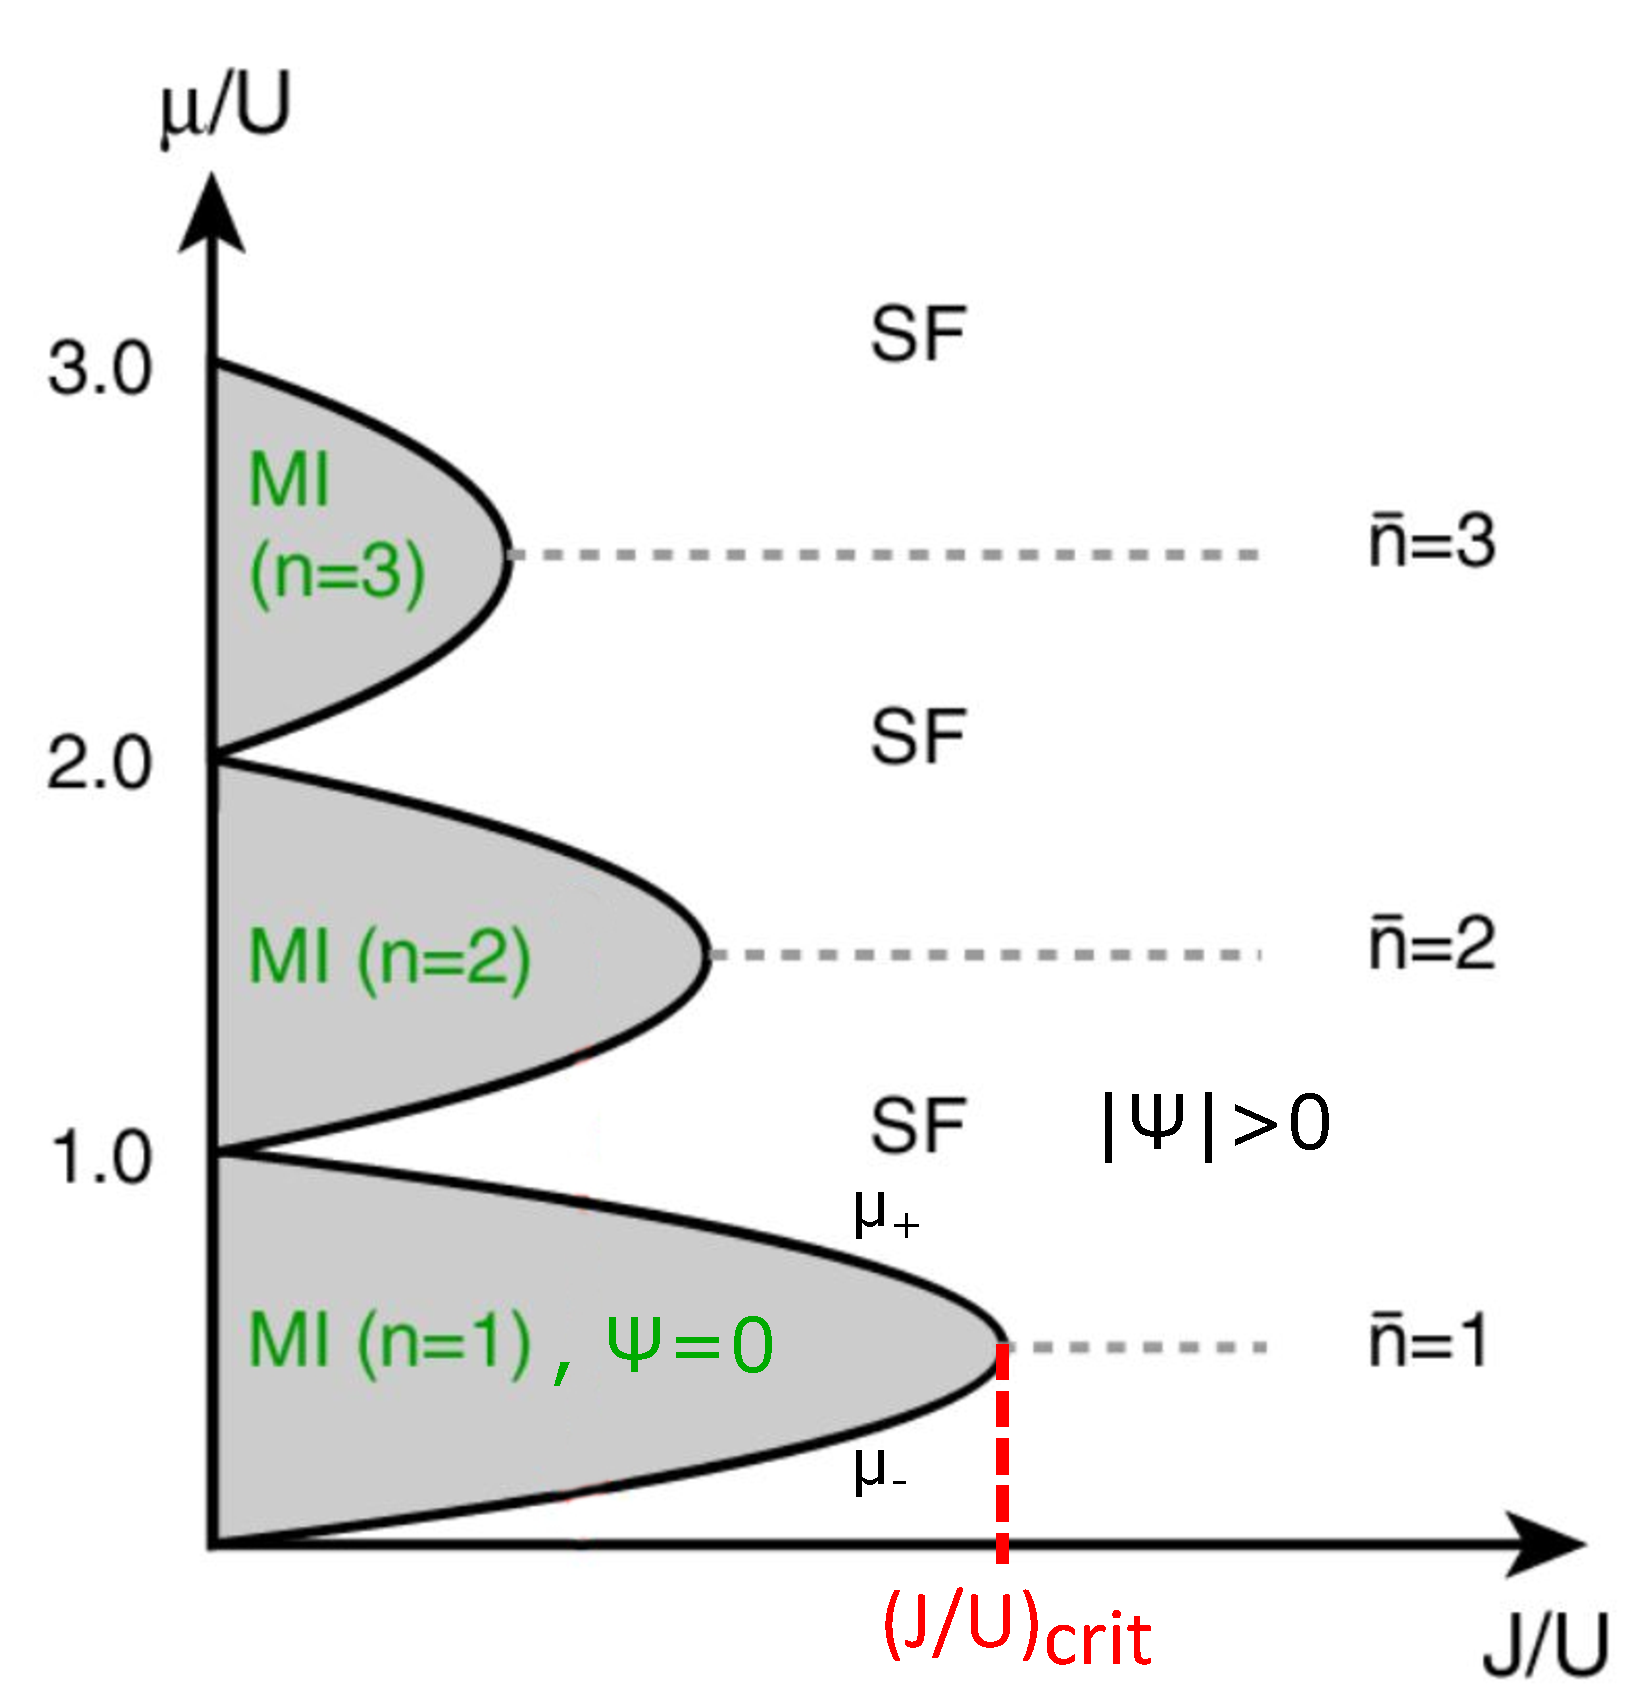
\includegraphics[width = 0.7\textwidth]{Figures/SFMottPhase.pdf}
	\label{fig:SFMOTT}
	\caption{\textit{Phase diagram of Bose-Hubbard model for T = 0. Grey areas mark the Mott Insulator phase for different number of particles per site, while white regions mark the superfluid phase. \cite{greiner}}}
\end{figure}
The $\mu_{\pm}$ curves encloses the region where the system is in the Mott Insulating phase. $(1/\bar{U})_{crit} = (J/U)_{crit}$ can be read off the graph from the point, where the two curves $\mu_{\pm}$ meet. As mentioned earlier, no fluctuations take place in the Mott Insulator, whereby the particle number per site is well defined, while it for the superfluid can take many values. As the chemical potential increases each site can accommodate more particles as long as the increase in chemical potential compensates the increased energy due to interactions between the particles.\\
The mean-field solution of the Bose-Hubbard model is only an approximation, which proves quite inaccurate for one dimension. This is seen when comparing the critical ratio for the mean-field approach, $\left( U/J \right)_{crit}^{MF,1D} = 11.66$, with numerical results computed using the DMRG method, $\left( U/J \right)_{crit}^{DMRG,1D} = 3.37$, \cite{Kuhner2000}. Nevertheless, it gives a good intuitive feeling of the physics taking place and how one can describe them without resorting to diagonalizing the Hamiltonian.\\